\subsection{Coherent Integration}

Using python and some inspiration from \cite{python_commpy}, a QAM16 constellation was generated (\inlinecodee{QAM\_constellation}). Each constellation point was copied $50$ times to simulate sampled data symbols which were then superimposed by normally distributed complex-valued noise. The noisy constellation diagram can be seen in figure \ref{fig:noisy_constellation}. The code can be found in appendix \ref{app:constellation}.

\begin{figure}[h]
  \centering
  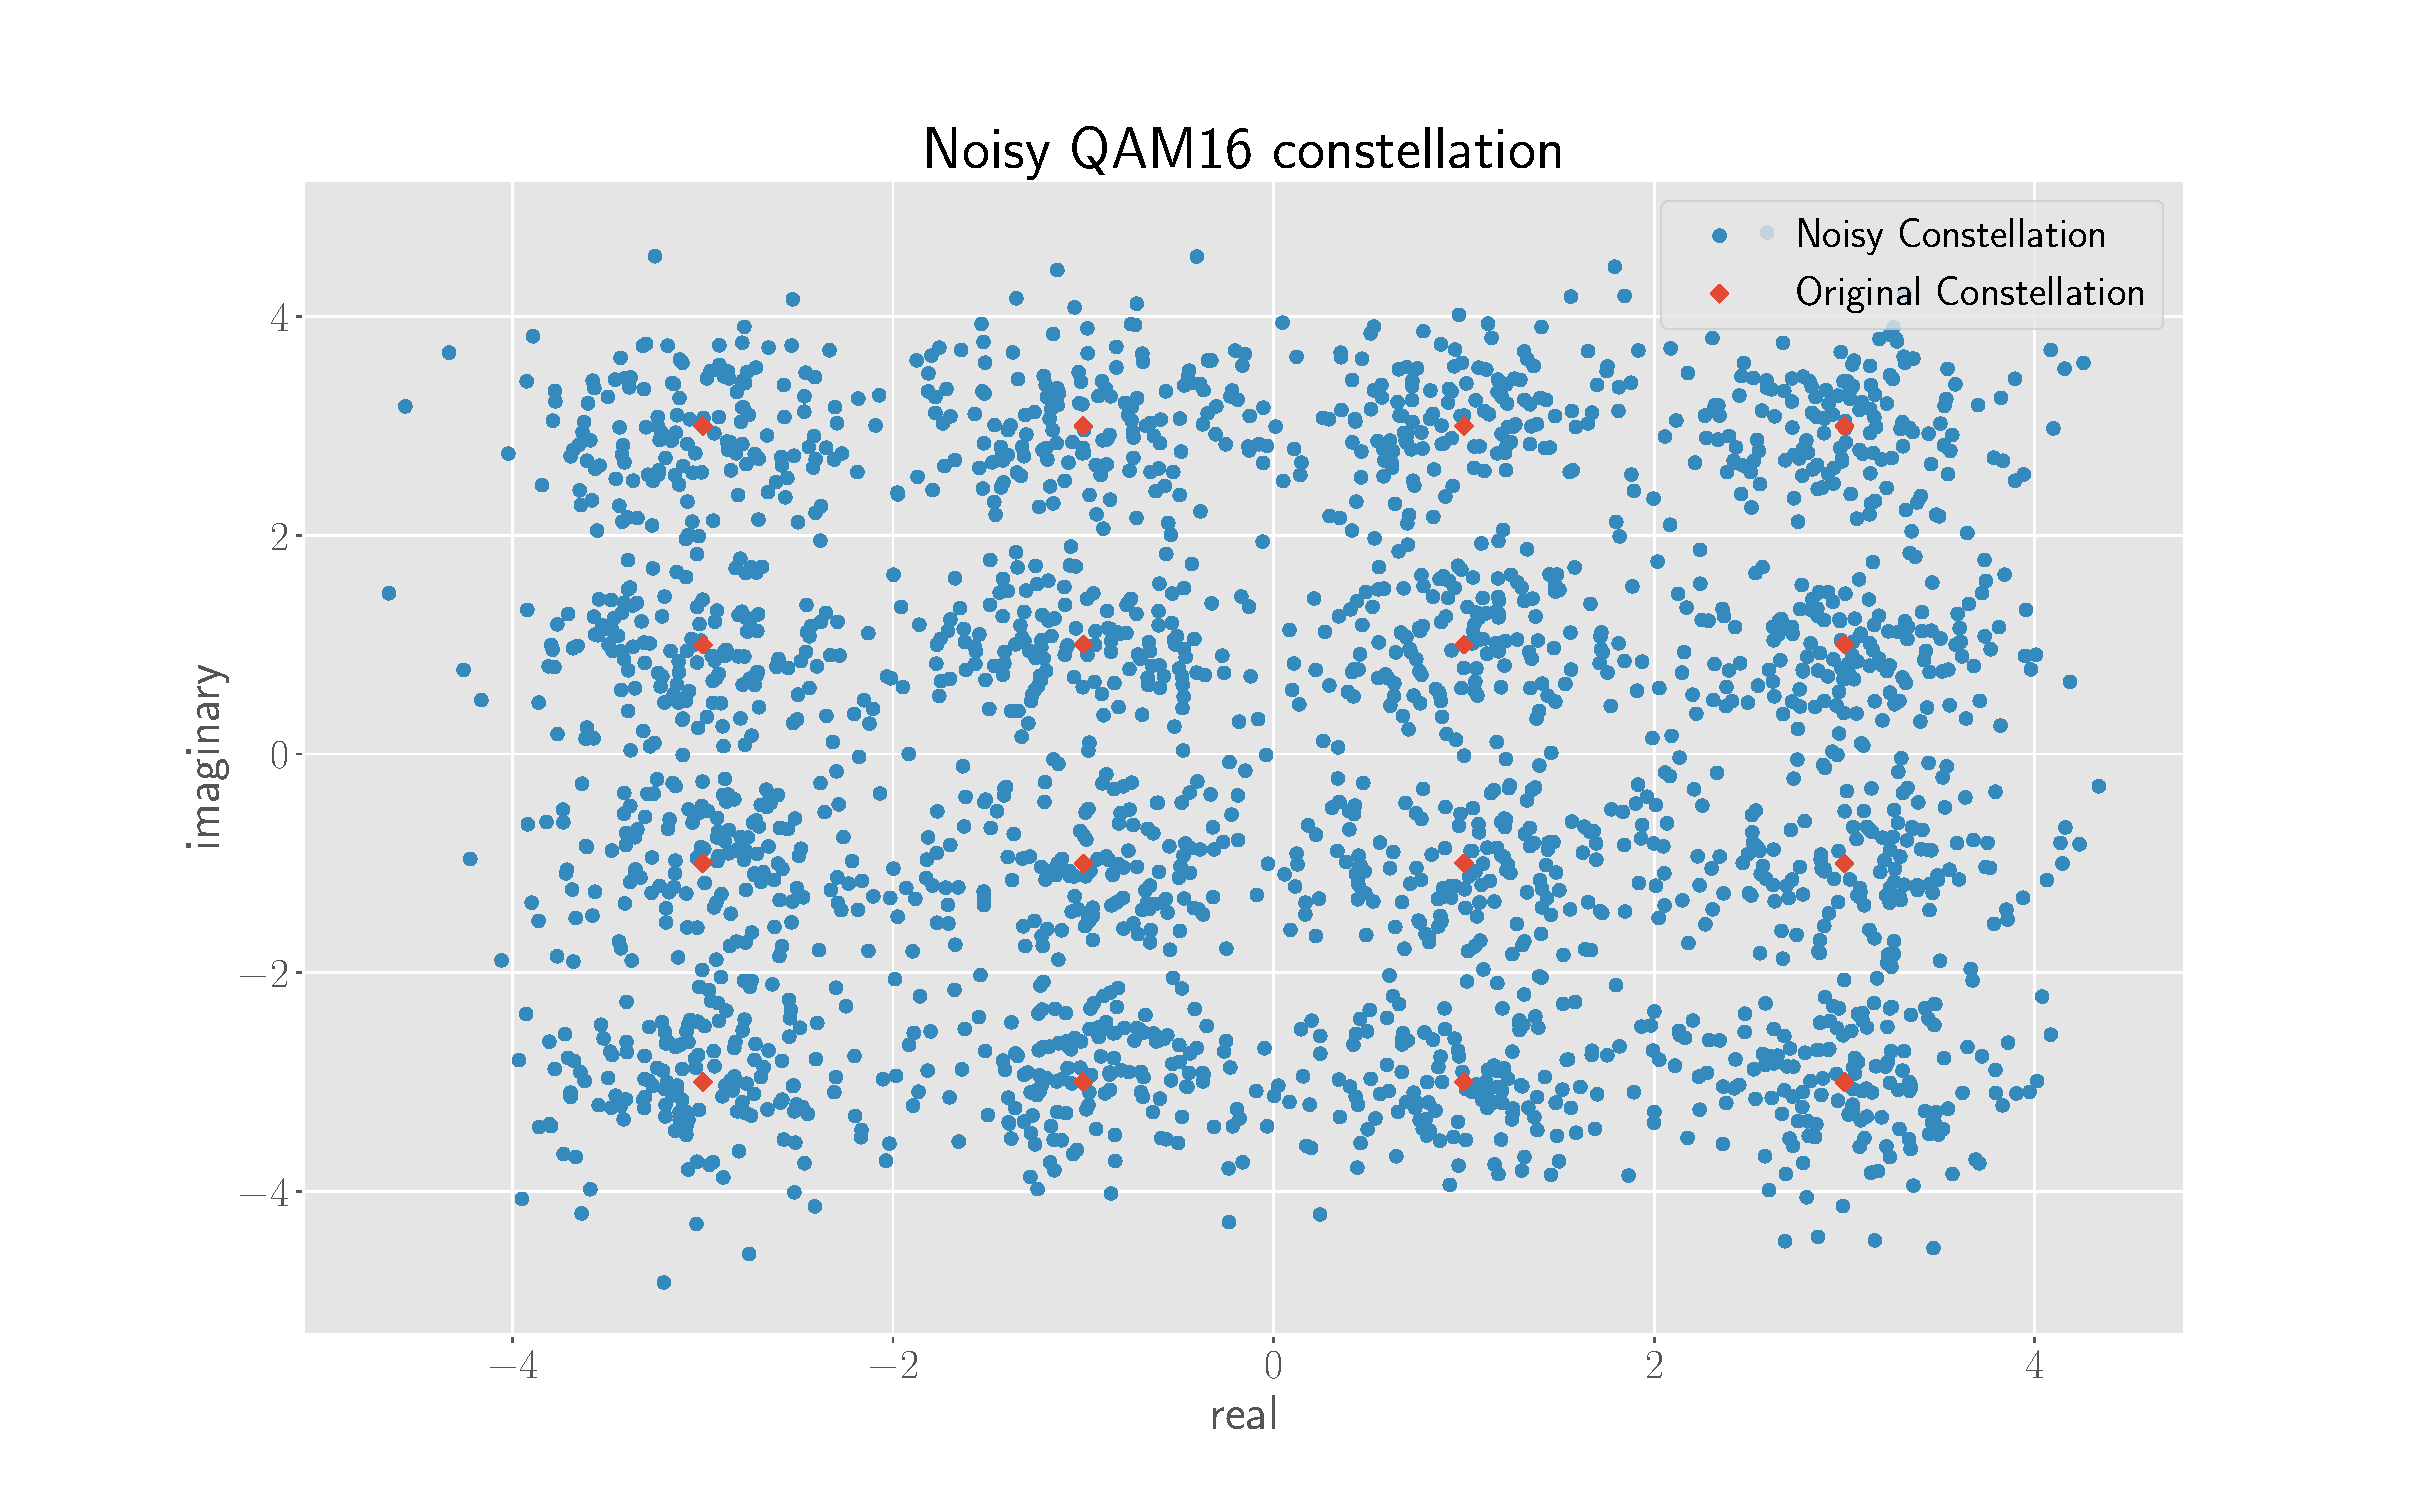
\includegraphics[width=0.763\textwidth]{graphics/constellation.pdf}
  \caption{Noisy constellation used as test data.}\label{fig:noisy_constellation}
\end{figure}


\subsection{Incoherent Integration}

For the incoherent integration, a sinusoidal signal with a frequency of $100\,\si{\hertz}$ was multiplied with a gaussian with standard deviation of $0.01\,\si{\second}$ to create a gaussian-shape spectrum centered around $100\,\si{\hertz}$. The center frequency of each realization was additionally superimposed by random jitter. The signal can be seen in figures \ref{fig:nci_signal}. Figure \ref{fig:nci_signal_spec} shows the realization spectra.

\begin{figure}
    \centering
    \begin{minipage}{0.5\textwidth}
        \centering
        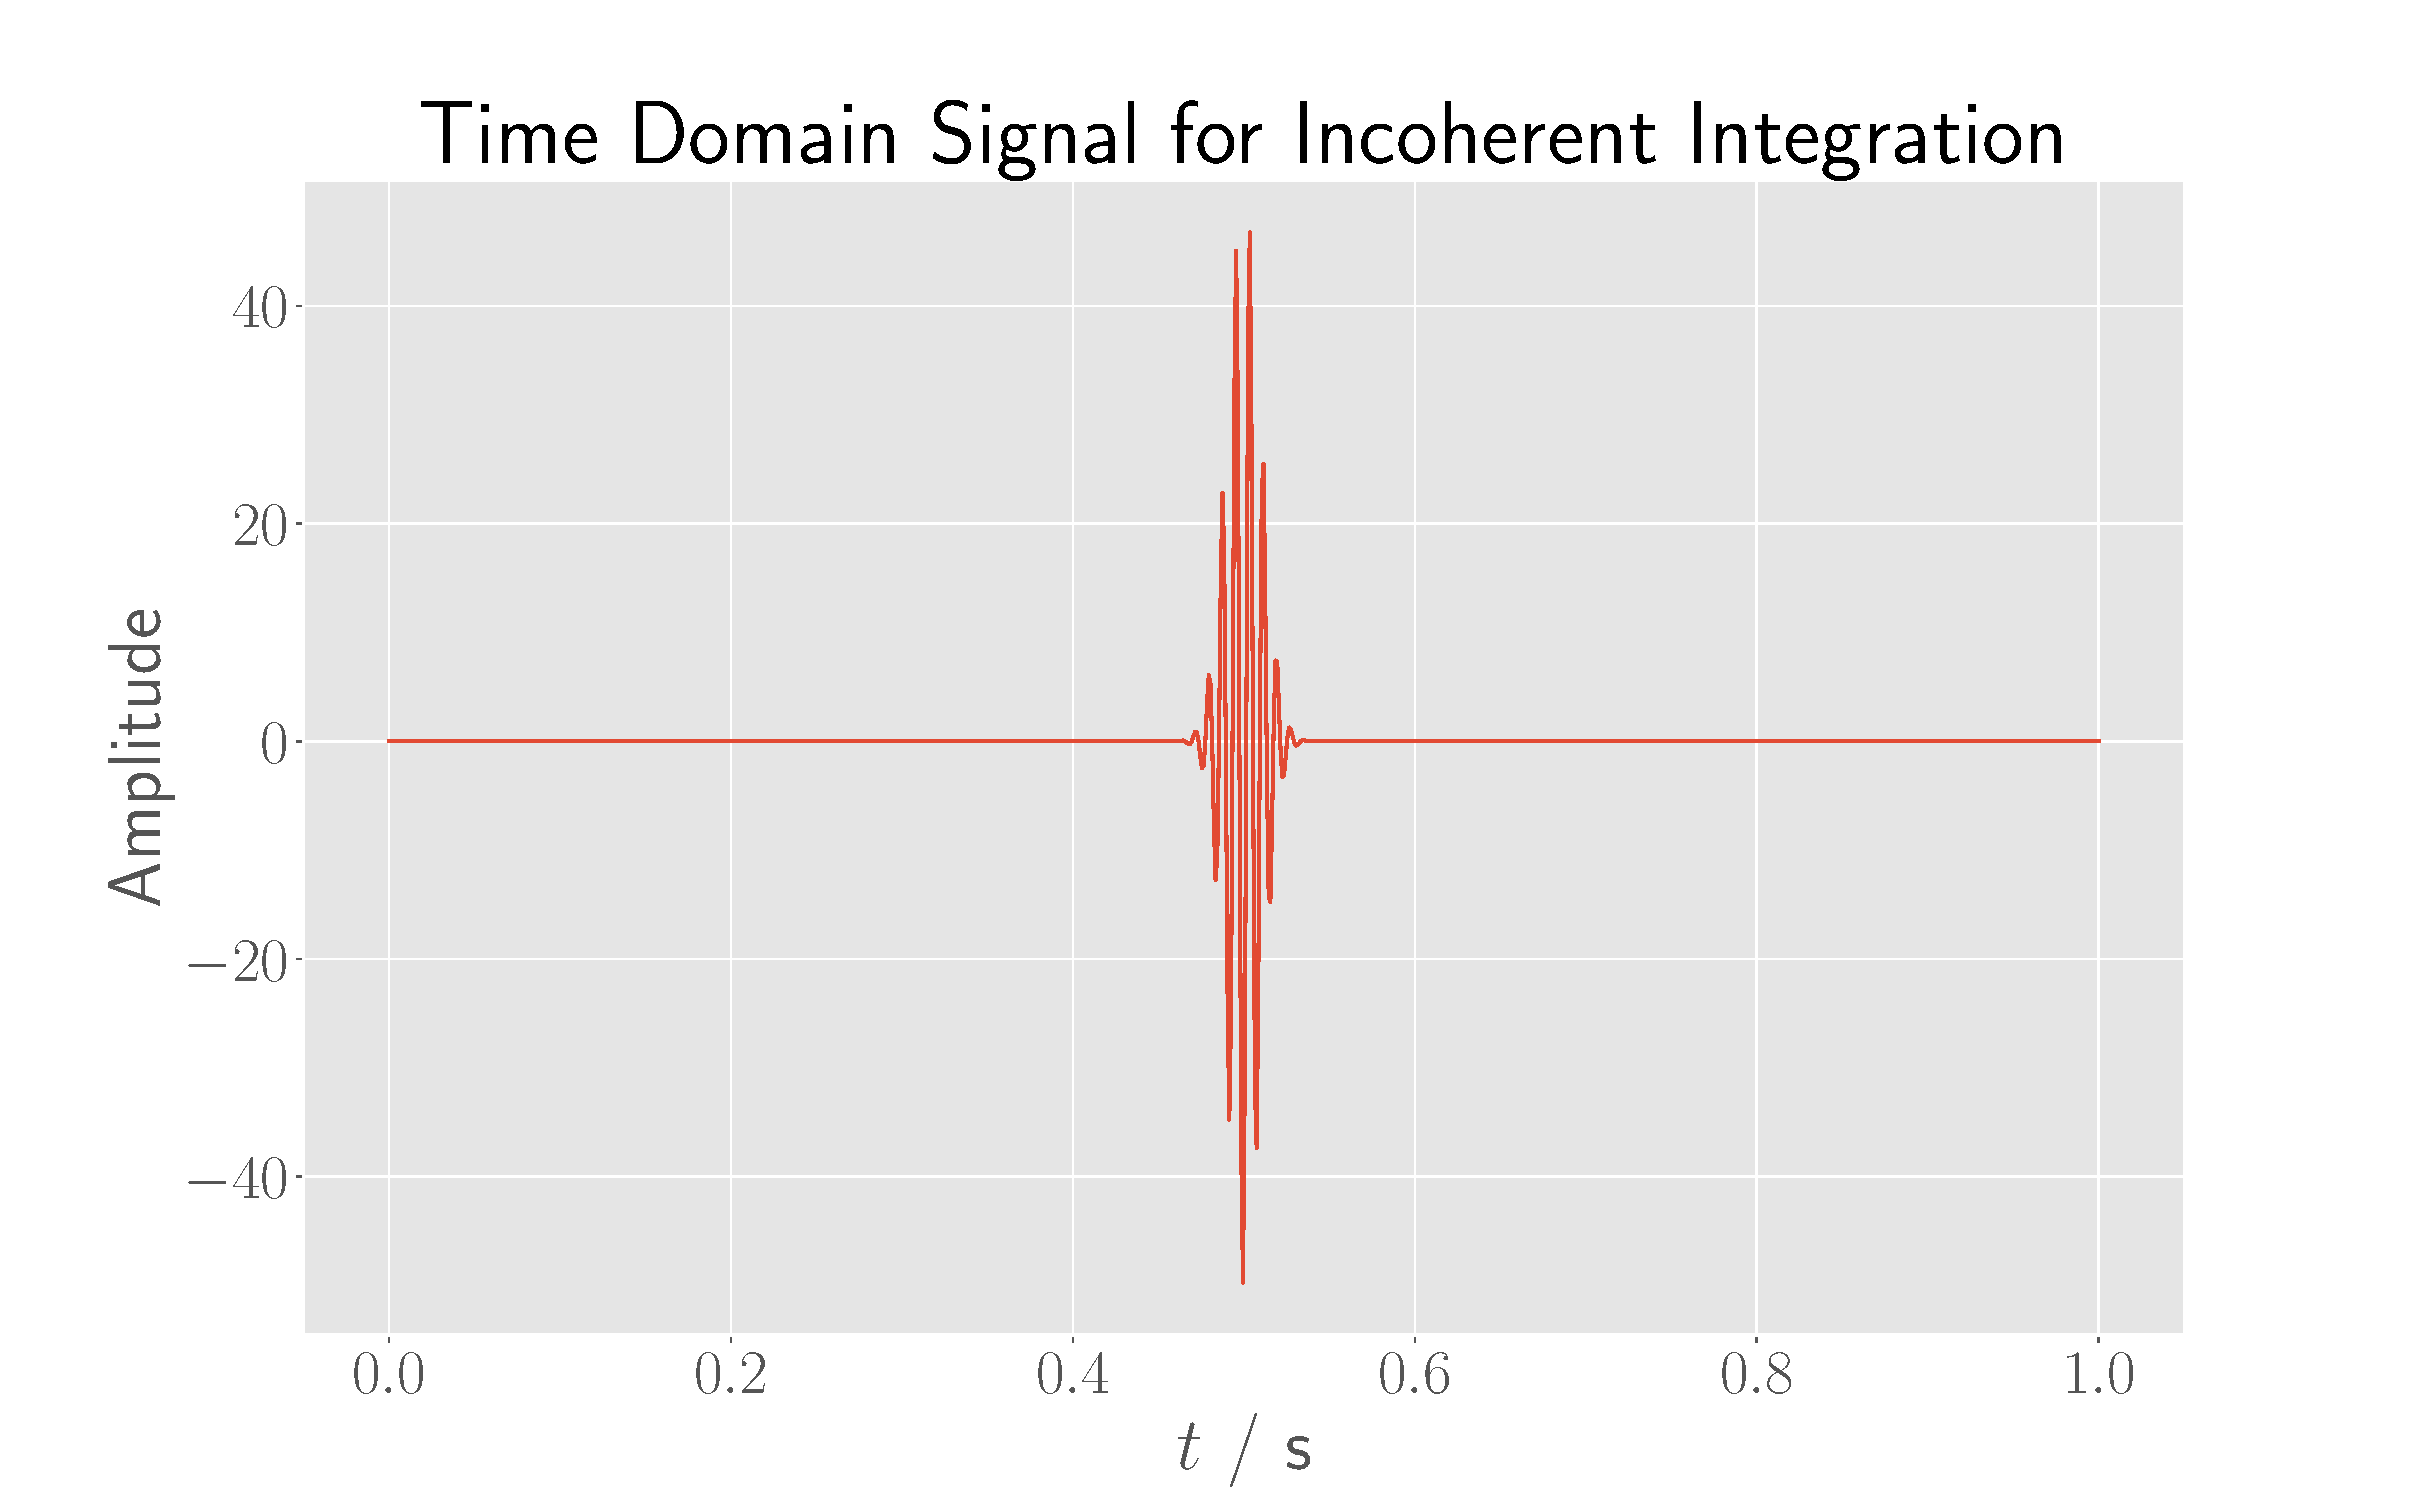
\includegraphics[width=1\textwidth]{graphics/nci_time.pdf} % first figure itself
        \caption{Time domain of NCI test signal (1 realization).}\label{fig:nci_signal}
    \end{minipage}\hfill
    \begin{minipage}{0.5\textwidth}
        \centering
        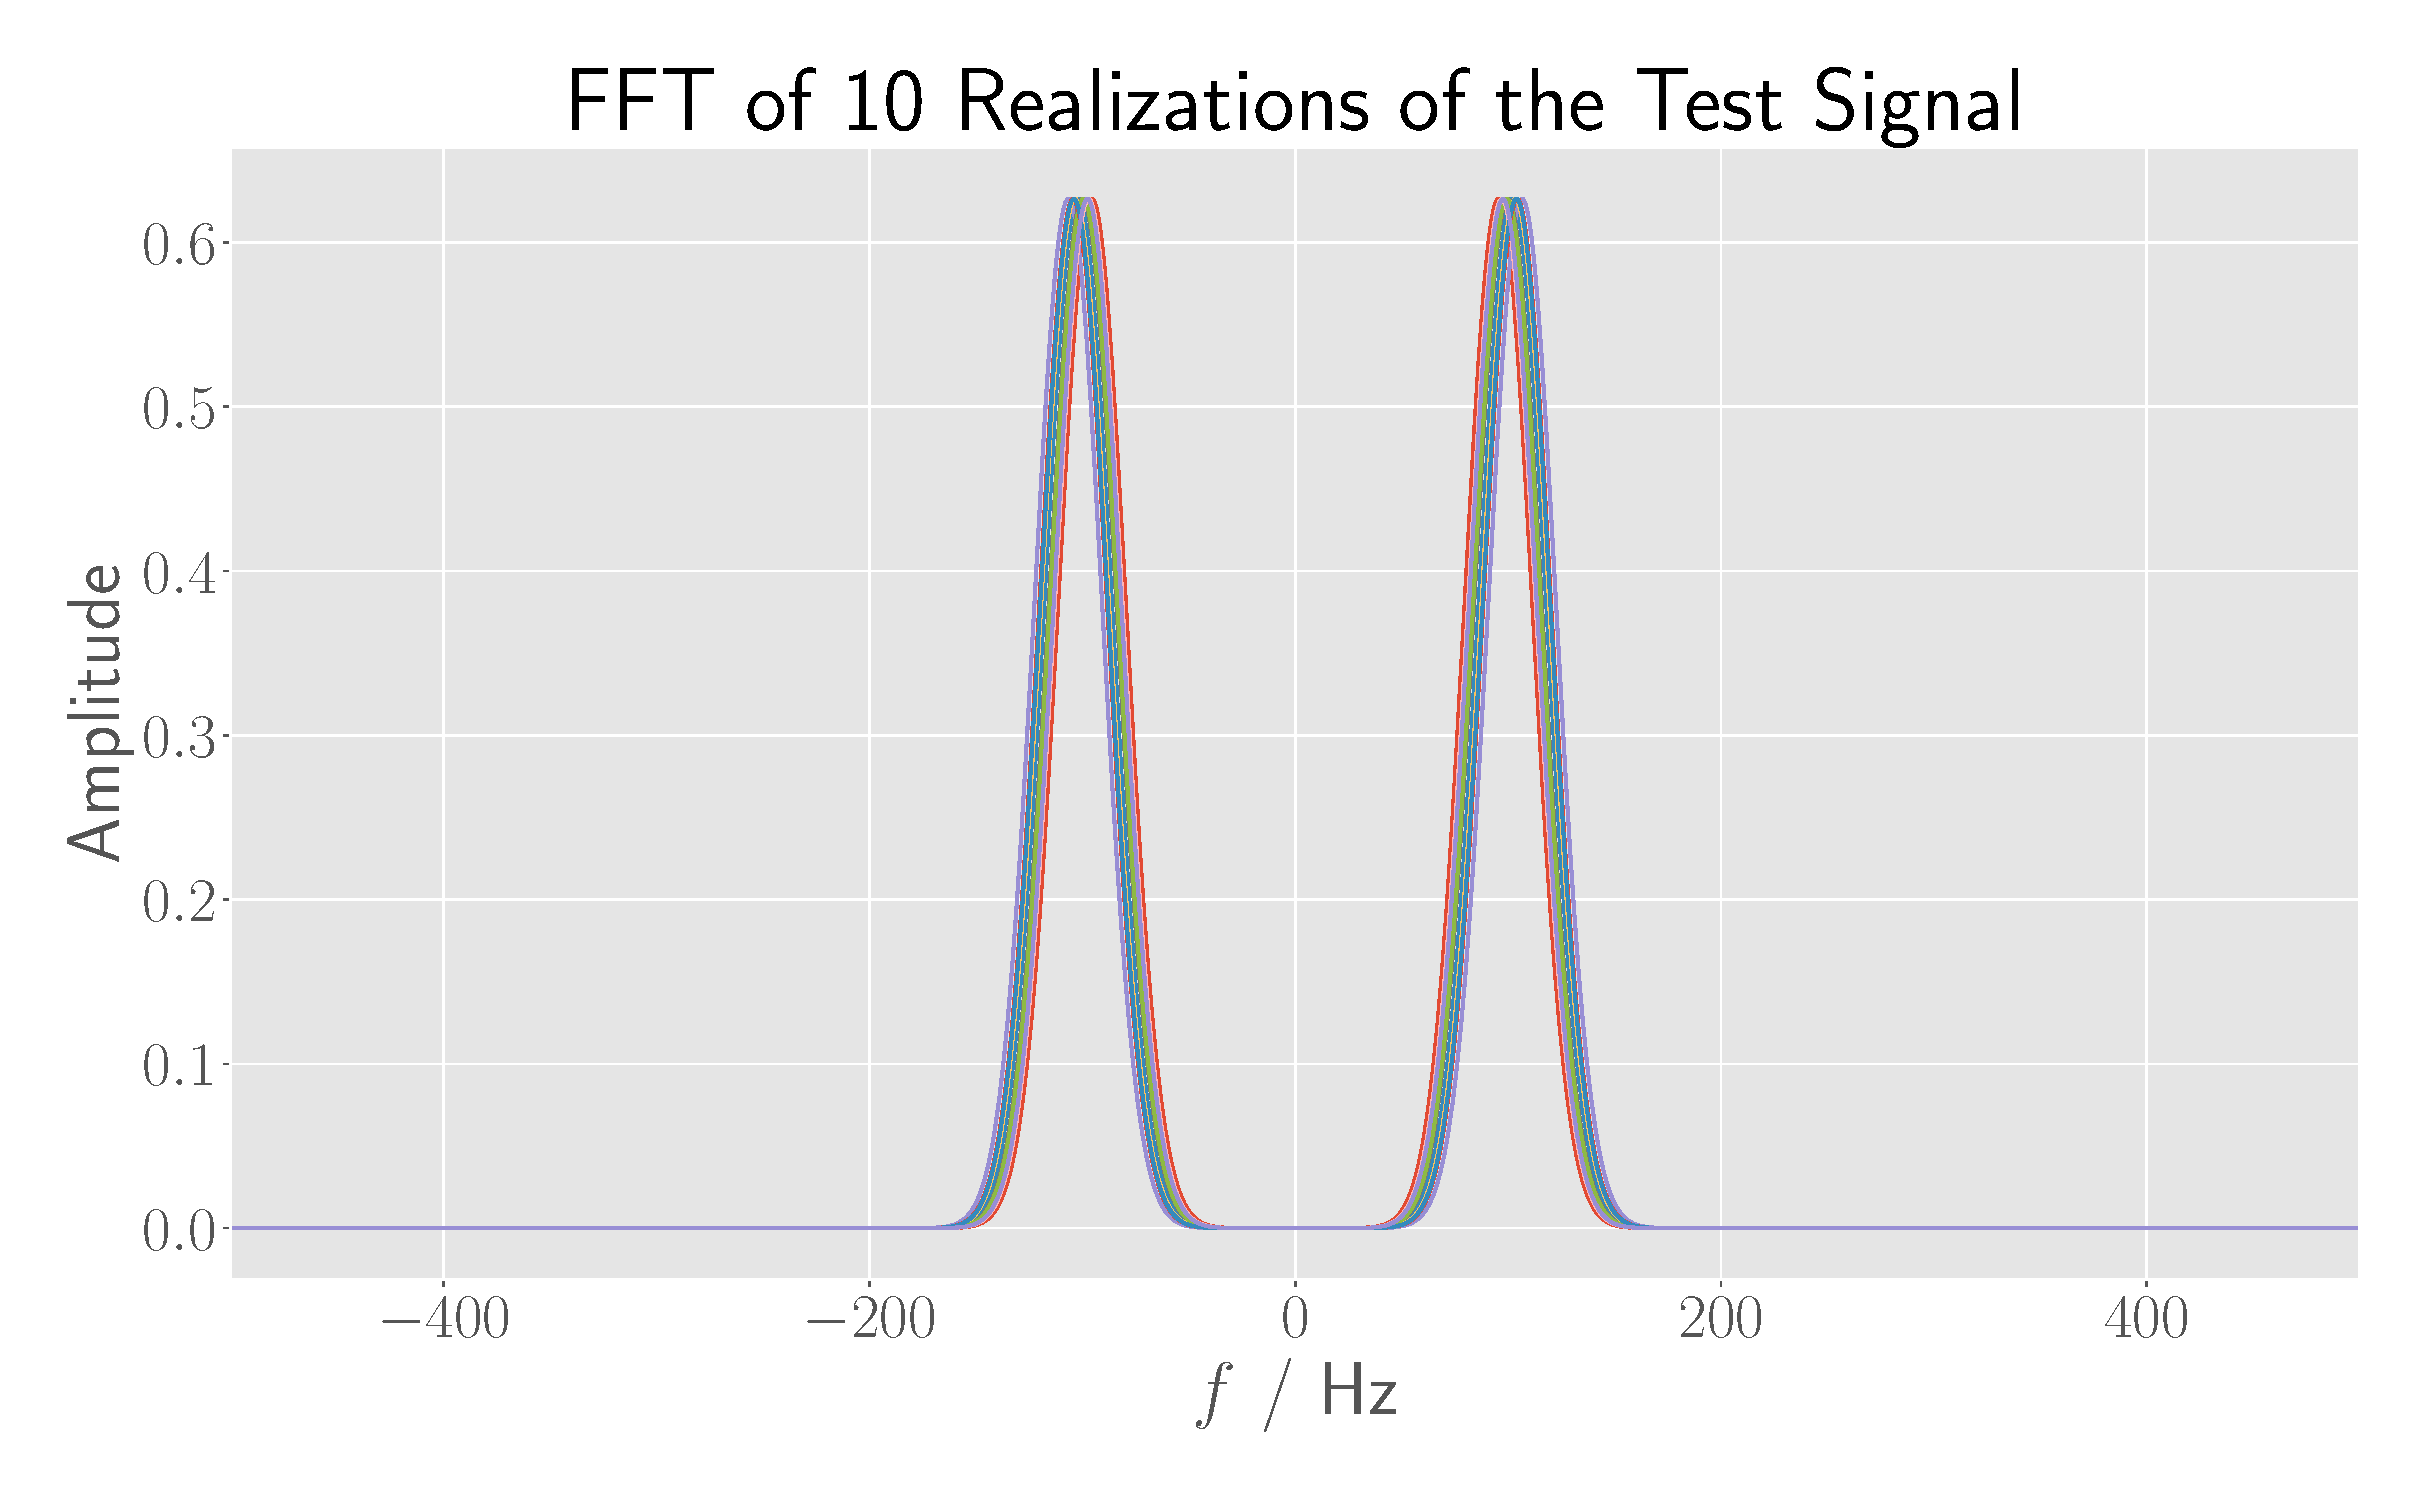
\includegraphics[width=1\textwidth]{graphics/nci_spec.pdf} % second figure itself
        \caption{FFTs of NCI test signals.}\label{fig:nci_signal_spec}
    \end{minipage}
\end{figure}

\subsection{Signal-To-Noise-Ratio}

For the coherent integration, the mean of the squared differences of each noisy sample towards their actual constellation points (the signal without the added noise) was calculated to obtain a measure of noise variance (power, $\sigma^{2}$). The square of the symbol distance ($1\,\si{\volt\squared}$) is then divided by this variance to get the SNR.\\

For incoherent integration, the definition of an SNR is more complicated. \cite{richards_pdf} Here, the SNR was approximated by taking the peak value of the averaged spectrum and dividing it by the noise power (standard deviation squared) which was taken from the first tenth of the spectrum.
